\graphicspath{{introduction/fig/}}

\chapter{Introduction}
\label{chap:introduction}

\section{Problem Statement and Project Objective}
In robotics, a manipulator (ie. a robotic arm) is a device used to manipulate objects in its environment. When the manipulation task is relatively complex, it is often difficult or even impossible for a human to direct how the robot should act. One possible solution is that the robot learn by itself which actions are best, which can be done through reinforcement learning. A popular method for doing developing reinforcement learning algorithms for robotics is to first solve similar, less complex problems.

In this project reinforcement learning is used to solve sliding puzzle. An example of a sliding puzzle being solved can be seen in Figure \ref{fig:sliding_puzzle_figs}. The objective of this project is to solve a shuffled puzzle with the minimum amount of moves using reinforcement learning. The rules of the game are explained in the next section, . 

\section{Background}

The sliding puzzle is a game with a history dating back to the 1870's. Many solutions have been thought up to solve such puzzles, which include using search algorithms\cite{search_alg}. The rules of the game are that the only tiles that can move are the ones next to the tile with no number, known as the 'blank tile'. Additionally only one tile can be moved at a time. The final puzzle configuration is shown in \ref{fig:sfig4}, where all the tiles are placed in ascending order read left to right and top to bottom. The aim of the game is to arrange a shuffled puzzle into the final puzzle configuration by moving one tile at a time.

\begin{figure}[!htb]
	\centering
	\begin{subfigure}{.4\textwidth}
		\centering
		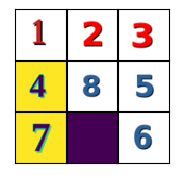
\includegraphics[width=.8\linewidth]{game_states/31.png}
		\caption{Puzzle with tiles 5,6,8 and blank in the incorrect positions}
		\label{fig:sfig1}
	\end{subfigure}%
	\begin{subfigure}{.4\textwidth}
		\centering
		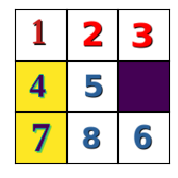
\includegraphics[width=.8\linewidth]{game_states/32.png}
		\caption{Puzzle with tiles 5,8 and blank in the incorrect positions}
		\label{fig:sfig2}
	\end{subfigure}
	\begin{subfigure}{.4\textwidth}
		\centering
		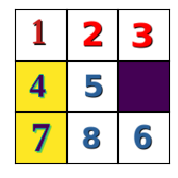
\includegraphics[width=.8\linewidth]{game_states/33.png}
		\caption{Puzzle with tiles 8 and blank in the incorrect positions}
		\label{fig:sfig3}
	\end{subfigure}
	\begin{subfigure}{.4\textwidth}
		\centering
		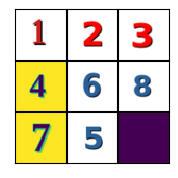
\includegraphics[width=.8\linewidth]{game_states/34.png}
		\caption{Solved puzzle}
		\label{fig:sfig4}
	\end{subfigure}
	\caption{Figures of a 3x3 sliding puzzle being solved}
	\label{fig:sliding_puzzle_figs}
\end{figure}

\section{Document Outline} 
Chapter \ref{chap:Literature_Review} looks at a paper which used an alternate approach to solve a 16 tile sliding puzzle.

Chapter \ref{chap:MDP} describes in detail the mathematical background theory which forms the basis for Reinforcement Learning.

Chapter \ref{chap:RL} discusses in detail the Reinforcement Learning techniques which will be used to solve our puzzle problem.

Chapter \ref{chap:System_Design} lays out the overarching view of the software system, broken down into functional blocks.

Chapter \ref{chap:Experiments_and_Results} contains tests and verification that our solution works using the results of various experiments.

Chapter \ref{chap:conclusion} concludes the report.